%% REPLACE SXXXXXX with your student number
\def\studentNumber{SXXXXXX}


%% START of YOUR ANSWERS
%% Add answers to the questions below, by replacing the text inside the brackets {} for \youranswer{ "Text to be replaced with your answer." }. 
%
% Do not delete the commands for adding figures and tables. Instead fill in the missing values with your experiment results, and replace the images with your own respective figures.
%
% You can generally delete the placeholder text, such as for example the text "Question Figure 2 - Replace the images ..." 
%
% There are 6 TEXT QUESTIONS. Replace the text inside the brackets of the command \youranswer with your answer to the question.
%
% There are also 2 "questions" to replace or add FIGURES, and 2 "questions" asking you to fill in missing TABLE entries or add a TABLE. The figures and tables in the problem identification section are provided.
%
% NOTE! that questions are ordered by the order of appearance of their answers in the text, and not by the order you should tackle them. You should complete the relevant experiments and fill in the TABLES and FIGURES before discussing the results presented there.
%
% NOTE! If for some reason you do not manage to produce results for some FIGURES and TABLES, then you can get partial marks by discussing your expectations of the results in the relevant TEXT QUESTIONS (for example Question 2 makes use of Table 3 and Figure 4).
%
% Please refer to the coursework specification for more details.


%% - - - - - - - - - - - - TEXT QUESTIONS - - - - - - - - - - - - 



%% Question 1:
\newcommand{\questionOne} {
\youranswer{Question 1 - Find and read the paper by Zou and Hastie (2005) specified in the coursework description. Explain na\"ive elastic net and its potential benefits. Cite the paper and provide relevant equations, considering both training and inference, explaining all variables and hyperparameters. Describe how you will implement this approach in PyTorch for the experiments in the next section.}
}

%% Question 2:
\newcommand{\questionTwo} {
\youranswer{Question 2 - Analyse and explain the results in Table~3 and Figure~4 on testing each regularization technique separately. While discussing na\"ive elastic net, mention how you decided on the hyperparameter values for it.
}
}

%% Question 3:
\newcommand{\questionThree} {
\youranswer{Question 3 - Using the supplied results and your experiments in Table~3, select and justify exactly \textbf{10} additional configurations varying the regularisation techniques and their hyperparameters. Select and justify all ten configurations before running them; sequential selection based on their results is not permitted. Follow the common experimental settings specified in the coursework description. These ten runs exclude the five runs needed to complete Table~3, the independent-method experiment in Question~5, and any necessary retraining for test evaluation. Run the ten experiments and present their results in Table~4 and Figure~5. You are assessed on your justification, correct experimental setup and execution, and analysis of the results, rather than on achieving high performance. Discuss the results in Question~4.}
}


%% Question 4:
\newcommand{\questionFour} {
\youranswer{Question 4 - Explain the experimental settings, including hyperparameters, and analyse the results in Tables~3 and~4 and Figures~4 and~5 in terms of generalisation performance and overfitting. Report epoch-100 results. Report ordinary cross-entropy against the original, unsmoothed labels, excluding all weight penalties. Follow the supplied notebook's convention for measuring training error and state that convention. Select the best configuration from Tables~3 and~4 using epoch-100 validation accuracy, using validation cross-entropy to break ties. Evaluate the selected model on the test set only after completing this selection, and report and discuss its test performance.}
}


%% Question 5:
\newcommand{\questionFive} {
\youranswer{Question 5 - Independently identify a regularisation approach other than dropout, L1, L2, na\"ive elastic net or label smoothing. Find and cite a research paper describing the approach. Explain its mechanism, relevant hyperparameters, and why it may help address overfitting in this task. Implement the approach in PyTorch and run one additional EMNIST experiment consisting of a single training run. Explain your implementation and justify your hyperparameter choices. Use the common architecture and training settings wherever compatible with the approach, explaining any necessary departures. Report validation accuracy, training and validation cross-entropy, and the generalisation gap, following the reporting conventions in the specification. Compare its validation results with those of the configuration selected in Question~4. Explain any differences in experimental settings that affect this comparison, and discuss the approach's benefits and limitations, recognising the limited evidence from one run. This experiment is additional to the ten runs required for Question~3.}
}

%% Question 6:
\newcommand{\questionSix} {
\youranswer{Question 6 - Briefly draw your conclusions based on the results from the previous sections (what are the take-away messages?), discussing them in the context of the overall literature, and conclude your report with a recommendation for future directions.}
}

%% - - - - - - - - - - - - FIGURES - - - - - - - - - - - - 

%% Question Figure 2:
\newcommand{\questionFigureTwo} {
    \begin{figure}[t]
        \centering
        \begin{subfigure}{\linewidth}
            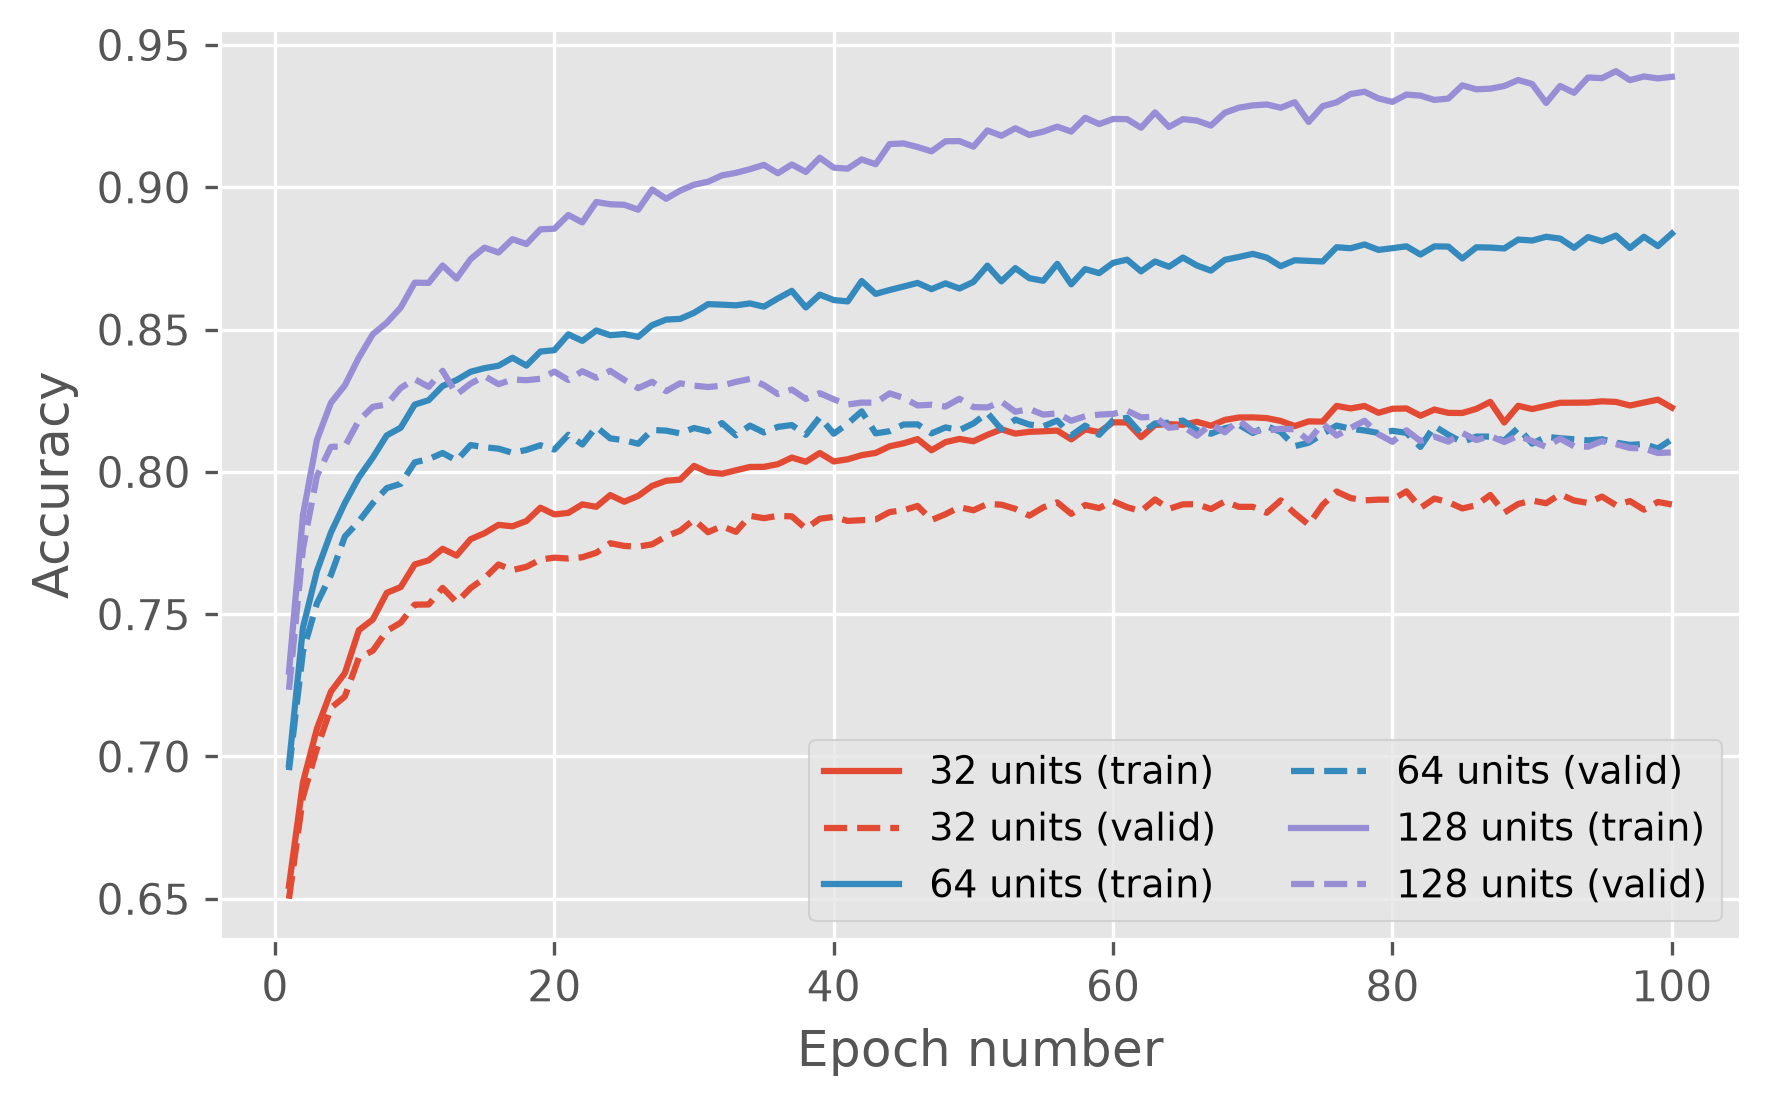
\includegraphics[width=\linewidth]{figures/fig2_width_accuracy.png}
            \caption{Accuracy by epoch.}
            \label{fig:width_acccurves}
        \end{subfigure}
        \begin{subfigure}{\linewidth}
            \centering
            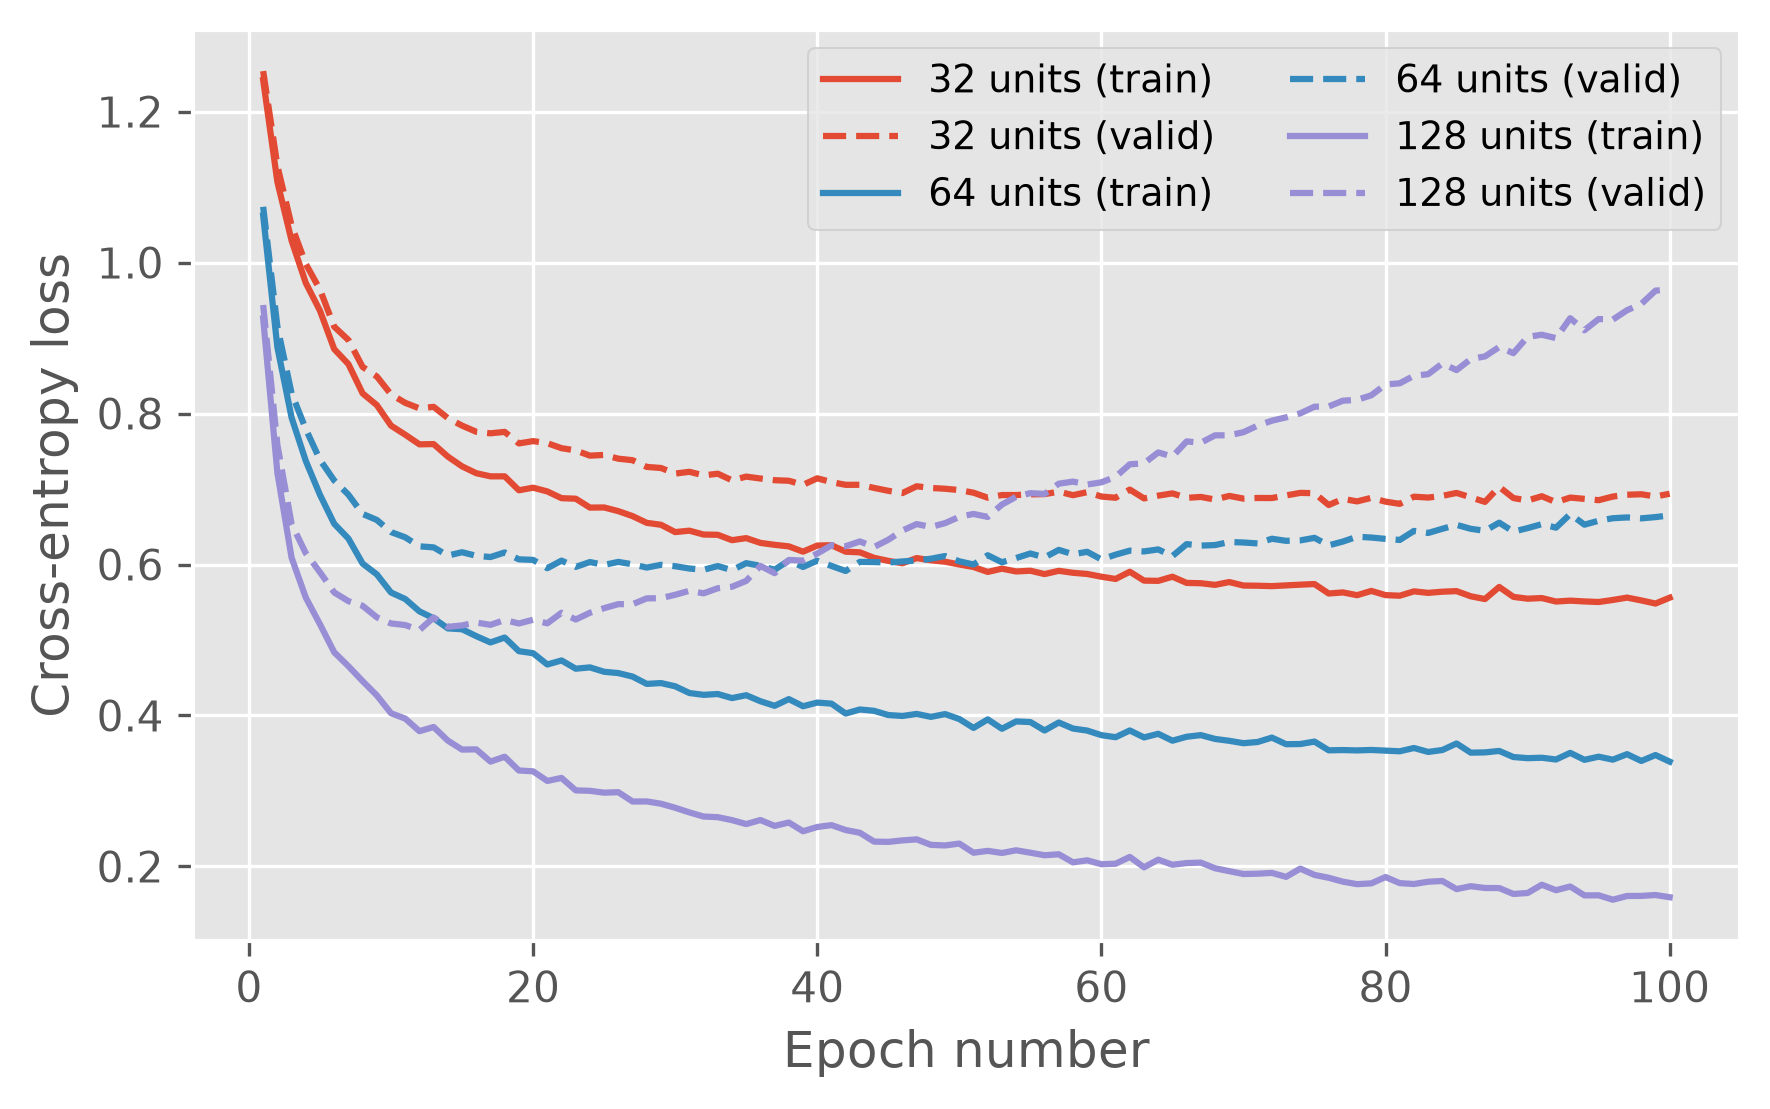
\includegraphics[width=\linewidth]{figures/fig2_width_loss.png}
            \caption{Cross-entropy by epoch.}
            \label{fig:width_errorcurves}
        \end{subfigure}
        \caption{Training (solid) and validation (dashed) accuracy and cross-entropy over 100 epochs for one-hidden-layer networks with 32, 64, or 128 ReLU units. }
        \label{fig:width}
    \end{figure}
}

%% Question Figure 3:
\newcommand{\questionFigureThree} {
    \begin{figure}[t]
        \centering
        \begin{subfigure}{\linewidth}
            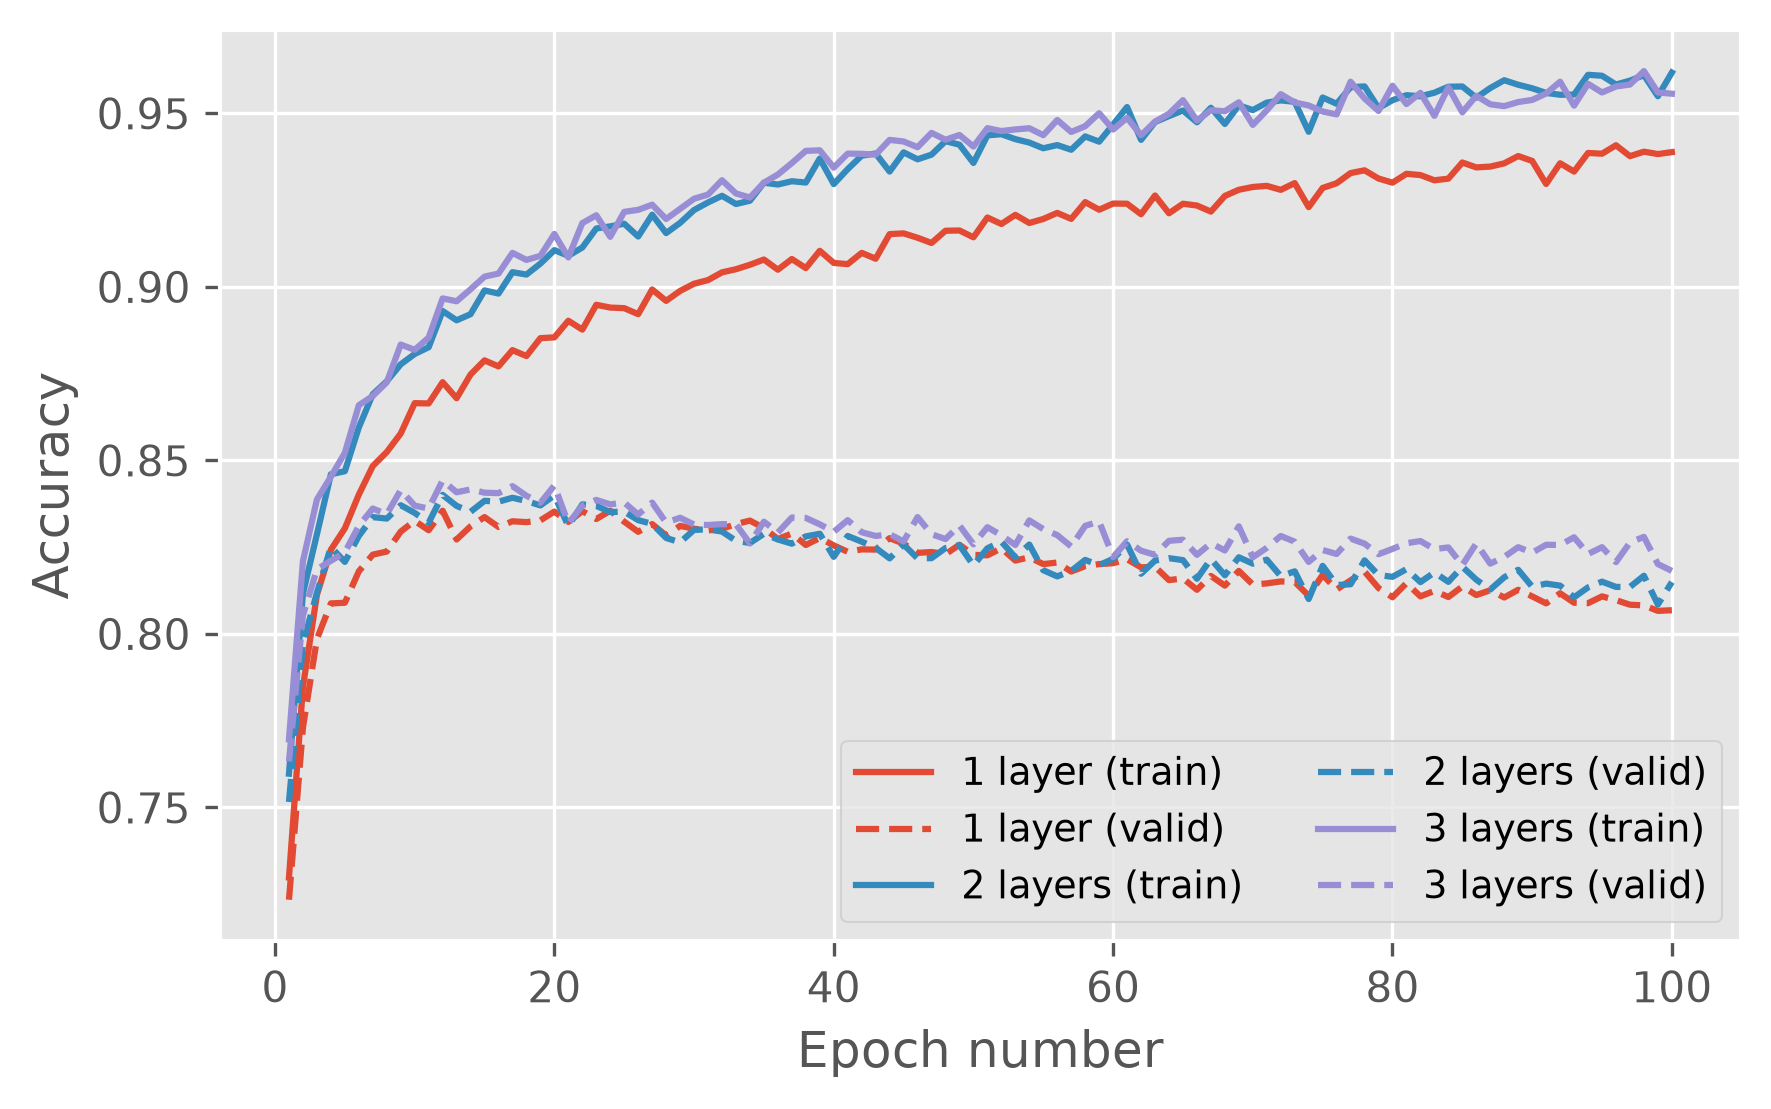
\includegraphics[width=\linewidth]{figures/fig3_depth_accuracy.png}
            \caption{Accuracy by epoch.}
            \label{fig:depth_acccurves}
        \end{subfigure}
        \begin{subfigure}{\linewidth}
            \centering
            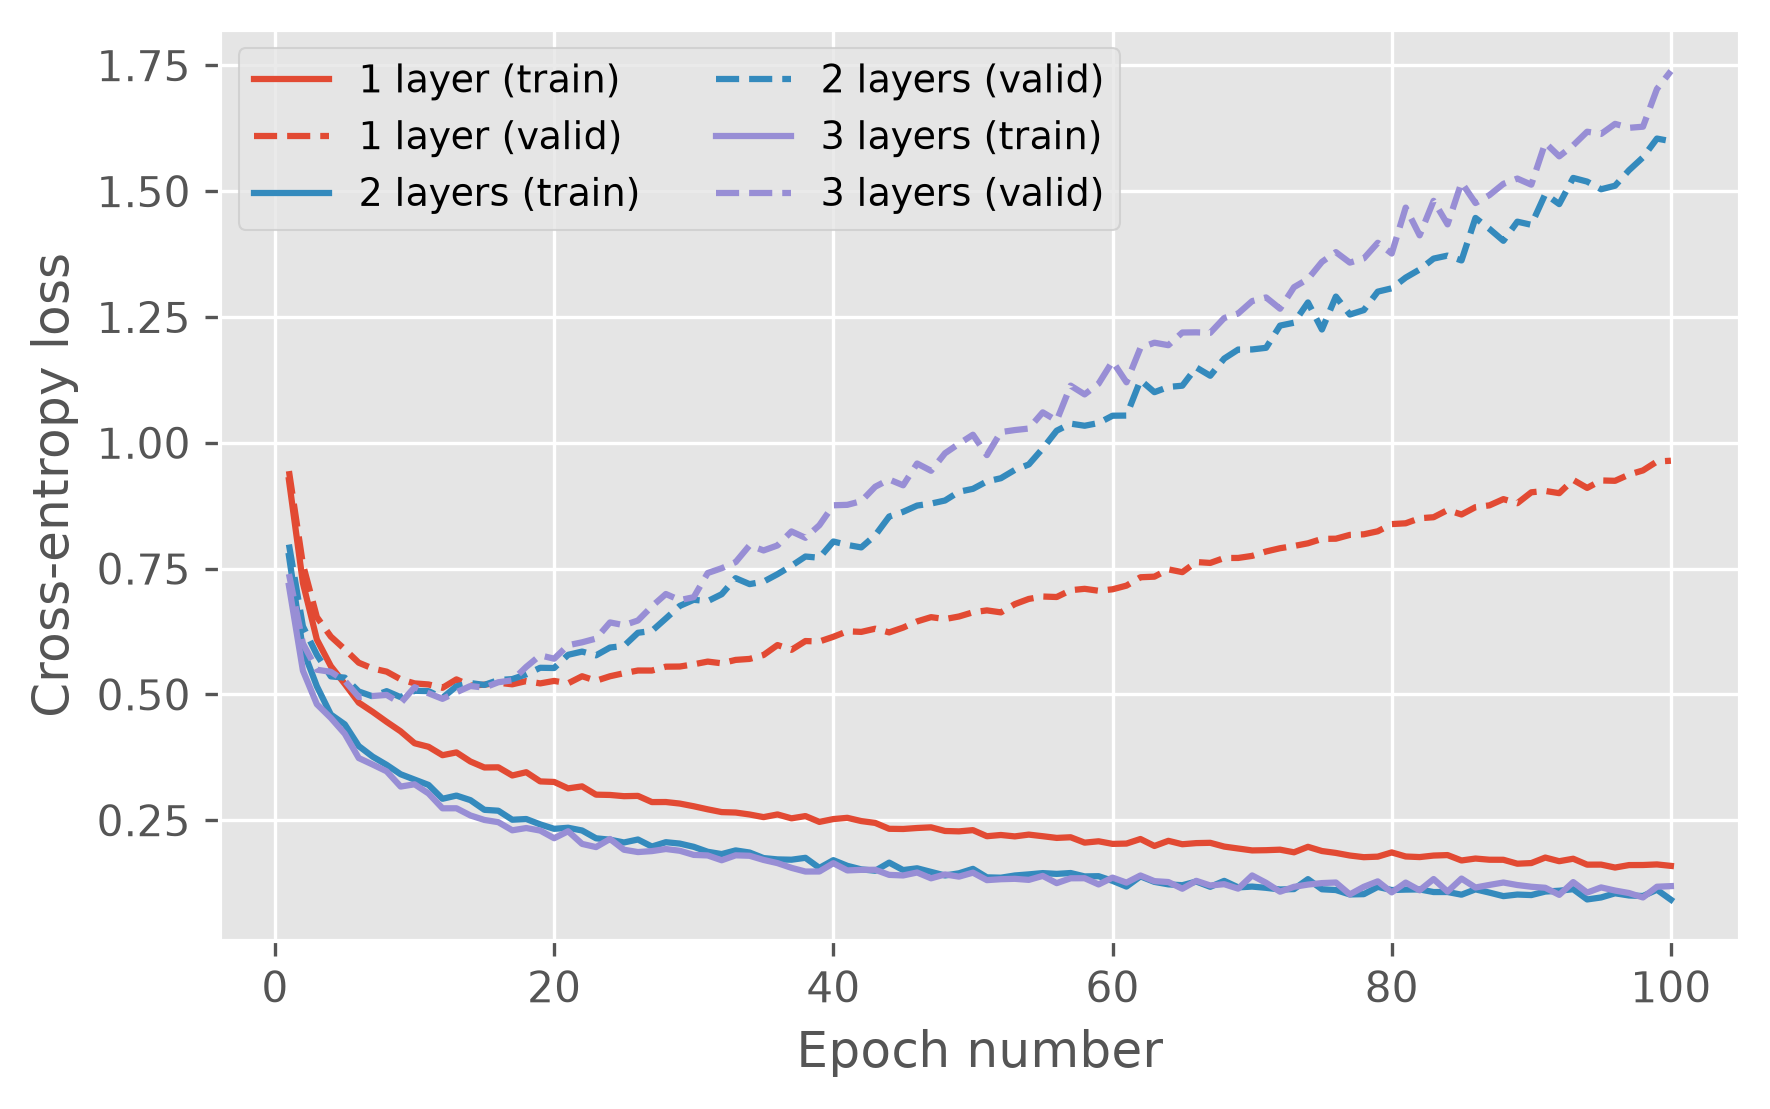
\includegraphics[width=\linewidth]{figures/fig3_depth_loss.png}
            \caption{Cross-entropy by epoch.}
            \label{fig:depth_errorcurves}
        \end{subfigure}
        \caption{Training (solid) and validation (dashed) accuracy and cross-entropy over 100 epochs for networks with one, two, or three ReLU hidden layers, each with 128 units.}
        \label{fig:depth}
    \end{figure}
}

%% Question Figure 4:
\newcommand{\questionFigureFour} {
\youranswer{Question Figure 4 - Replace these images with figures depicting the Validation Accuracy and Generalisation Gap (difference between validation and training error) for each of the experiment results varying the Dropout inclusion rate, and L1/L2 weight penalty depicted in Table 3 (including any results you have filled in).
%
\begin{figure*}[t]
    \centering
    \begin{subfigure}{.475\linewidth}
        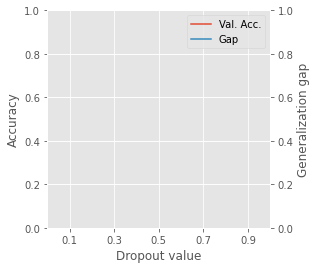
\includegraphics[width=\linewidth]{figures/empty_dropout_plot.png}
        \caption{Validation accuracy and generalisation gap by inclusion probability.}
        \label{fig:dropoutrates}
    \end{subfigure} 
    \begin{subfigure}{.475\linewidth}
        \centering
        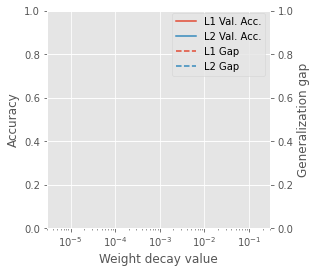
\includegraphics[width=\linewidth]{figures/empty_wd_plot.png}
        \caption{Validation accuracy and generalisation gap by penalty coefficient.}
        \label{fig:weightrates}
    \end{subfigure} 
    \caption{Epoch-100 validation accuracy and generalisation gap (validation minus training cross-entropy) against regularisation strength for dropout and L1/L2 regularisation.}
    \label{fig:hp_search}
\end{figure*}
}
}

%% Question Figure 5:
\newcommand{\questionFigureFive} {
\youranswer{Question Figure 5 - Add figures depicting the Validation Accuracy and Generalisation Gap (difference between validation and training error) for each of your 10 experiments depicted in Table 4.
}
}

%% Question Figure 6:
% \newcommand{\questionFigureSix} {
% \youranswer{Question Figure 6 - Add figures depicting the Training Accuracy, Error, and Gradient Flow Across Parameter Tensors for the one experiment run with the provided custom activation (produce these by running the "Problematic Training" cell in the Coursework\_1.ipynb notebook).
% }
% }

%% - - - - - - - - - - - - TABLES - - - - - - - - - - - - 

%% Question Table 1:
\newcommand{\questionTableOne} {
    \begin{table}[t]
        \centering
        \begin{tabular}{c|ccc}
        \toprule
        \# Hidden Units & Val. Acc. & Train Error & Val. Error \\
        \midrule
        32 & 78.9 & 0.556 & 0.694 \\
        64 & 81.1 & 0.339 & 0.665 \\
        128 & 80.7 & 0.159 & 0.964 \\
        \bottomrule
        \end{tabular}
        \caption{Epoch-100 validation accuracy (\%) and training/validation cross-entropy for one-hidden-layer ReLU networks on EMNIST.}
        \label{tab:width_exp}
    \end{table}
}

%% Question Table 2:
\newcommand{\questionTableTwo} {
    \begin{table}[t]
        \centering
        \begin{tabular}{c|ccc}
        \toprule
        \# Hidden Layers & Val. Acc. & Train Error & Val. Error \\
        \midrule
        1 & 80.7 & 0.159 & 0.964 \\
        2 & 81.5 & 0.092 & 1.599 \\
        3 & 81.8 & 0.119 & 1.739 \\
        \bottomrule
        \end{tabular}
        \caption{Epoch-100 validation accuracy (\%) and training/validation cross-entropy for ReLU networks with 128 units per hidden layer on EMNIST. Adam learning rate $10^{-3}$, batch size 100, seed 111020.}
        \label{tab:depth_exps}
    \end{table}
}

%% Question Table 3:
\newcommand{\questionTableThree} {
\youranswer{
Question Table 3 - Fill in Table 3 with the results from your experiments for the missing hyperparameter values for each of L1 regularisation, L2 regularisation, Dropout and label smoothing (use the values shown on the table). For Na\"ive Elastic Net, you need to implement the technique, choose an appropriate set of hyperparameter values, and report the results of one experiment in the table.
%
\begin{table*}[t]
    \centering
    \begin{tabular}{c|c|ccc}
    \toprule
        Model    &  Hyperparameter value(s) & Validation accuracy (\%) & Train Error & Validation Error \\
    \midrule
    \midrule
        Baseline &  -                    & 84.0 & 0.242 & 0.530 \\
    \midrule
        \multirow{4}*{Dropout}
                 & 0.6                   & 81.7 & 0.487 & 0.551 \\
                 & 0.7 & --.- & -.--- & -.---  \\
                 & 0.85 & 85.2 & 0.305 & 0.429 \\
                 & 0.97 & 85.6 & 0.229 & 0.447 \\
    \midrule
        \multirow{4}*{L1 penalty}
                 & 5e-4 & 79.6 & 0.643 & 0.663 \\
                 & 1e-3 & --.- & -.--- & -.--- \\
                 & 5e-3 & 2.19 & 3.850 & 3.850 \\
                 & 5e-2 & 2.13 & 3.850 & 3.850 \\
    \midrule
        \multirow{4}*{L2 penalty}  
                 & 5e-4 & 84.6 & 0.312 & 0.460 \\
                 & 1e-3 & --.- & -.--- & -.--- \\
                 & 5e-3 & 81.7 & 0.579 & 0.601 \\
                 & 5e-2 & 44.2 & 2.117 & 2.118 \\
    \midrule
        Label smoothing & 0.1 & --.- & -.--- & -.--- \\
    \midrule
        Na\"ive Elastic Net & --.- & --.- & -.--- & -.--- \\
    \bottomrule
    \end{tabular}
    \caption{Results of the individual-method experiments.
Report epoch-100 results, matching the supplied entries,
with random seed 111020. Errors are ordinary cross-entropy
against the original, unsmoothed labels and exclude all
weight penalties. \emph{Italics} indicate the best configuration
for each method (dropout, L1 regularisation, L2 regularisation,
label smoothing and na\"ive elastic net), and \textbf{bold}
indicates the best configuration in this table. Rank
configurations by validation accuracy, using validation
cross-entropy to break ties.}
    \label{tab:hp_search}
\end{table*}
}
}


%% Question Table 4:
\newcommand{\questionTableFour} {
\youranswer{
Question Table 4 - Add a table with the results from your 10 experiments (by which we mean: 10 training runs, NOT 10 sets of experiments) varying different hyper-parameters and regularization combinations.
}
}

%% END of YOUR ANSWERS
